\subsection{BXtend}
\label{sec:BXtend}

\NOTE{\emph{Solution expert:} Thomas, \emph{Interviewer:} Tony}

% Intro

BXtend~\cite{MODELSWARD2018-Buchmann}, short for \emph{Bidirectional Xtend}, is a pragmatic approach to programming bidirectional transformations resulting from years of experience trying to apply existing bx languages to solve realistic problems~\cite{DBLP:conf/icsoft/BuchmannG16}.
While bx languages might be theoretically more productive due to their formal guarantees (e.g., correctness), or because one only needs to specify one synchronization direction and gets the other for free, any possible gain in productivity might be substantially outweighed in practice by other, more mundane concerns: bx language are often \emph{exotic} in the sense that they are unfamiliar and thus difficult to learn for the average programmer; bx languages are also often (severely) limited in expressiveness -- while chosen simple examples might work beautifully with the language, realistic problems require a considerable amount of pre- and postprocessing effectively nullifying any other advantages of the language.

BXtend focuses on supporting bx \emph{best practices}, i.e., effective techniques with which synchronization problems can be solved in a standard programming language.
Xtend\footnote{\url{www.eclipse.org/xtend}} is used as a modern language as it provides a concise syntax, modern features, and a seamless integration with the Eclipse IDE and the mainstream programming language Java.
While BXtend does not give any formal guarantees or support automated inference of parts of required programs, it provides a framework in which developers can structure their bx solutions in a straightforward manner.
Typical auxiliary tasks are supported via a growing library of helper functions and numerous conventions can be followed to simplify the conceptual task of implementing a consistent pair of synchronizers.

\subsubsection{Classification}

BXtend's architectural style is \emph{restoration-based}, addressing \emph{initial-diag-based} application scenarios (see table~\ref{tab:features-all-tools}).
The restoration-based architecture for initial-diag-based application scenarios is depicted to the left of figure~\ref{fig:initialDiagBased}:  the programmer takes a diag and has the task of manipulating the dependent model until both models are consistent again.
The corr between the models should also be updated in the process and returned.

With BXtend, the program representing \emph{fCR/bCR} is decomposed into multiple ``rules'' consisting of restoration logic separated into forward and backward direction.
Each rule defines flexibly, e.g., based on a certain type, if it is applicable and can be used to check and fix a specific inconsistency or not.
Similarly, each rule checks first by exploiting the supplied diag if existing structure in the dependent model can be reused, suitably changed, or must be deleted and created as required.
To perform \emph{fCR/bCR} on the top-most level, an orchestration component is implemented to decide the order in which individual rules are applied and combined to realize \emph{fCR/bCR}.
This global component can also perform a final clean up if required.
The delta implicitly induced as output (see figure~\ref{fig:initialDiagBased}) is mixed in the sense that each rule can already perform deletion and creation as required.

BXtend provides no formal guarantees: both synchronization directions are implemented separately and are free to contradict each other.
This can be viewed positively: the bx programmer is free to do whatever is required to solve the current task.
%
There is no explicitly specified notion of consistency, i.e., this is \emph{implicitly} given by the implemented pair of \emph{fCR/bCR}.
%
Synchronization is performed \emph{on-demand}, and is completely explicit, i.e., the bx developer implements both \emph{fCR} and \emph{bCR} explicitly in Xtend.

\subsubsection{Benchmark solution with BXtend}

To provide an impression of the benchmark solutin with BXtend, figure~\ref{fig:bxtendSoln} depicts two classes:  \texttt{Family\-2\-Person\-Transformation} representing the orchestrating component, and \texttt{Mother\-Daughter\-2\-Female} representing a BXtend rule.
For the Families-to-Persons benchmark, the same ordering of rules can be used in both directions (see label~1).
This order is specified in \texttt{addRules()}; three rules are created and added following the composition hierarchy of the metamodels (first containers then containees).
While the bx developer is free to program arbitrarily complex rule orchestration, current experience indicates that such a fixed order along the composition hierarchy is sufficient in most cases.

\begin{figure}[!tbp]
    \centering
    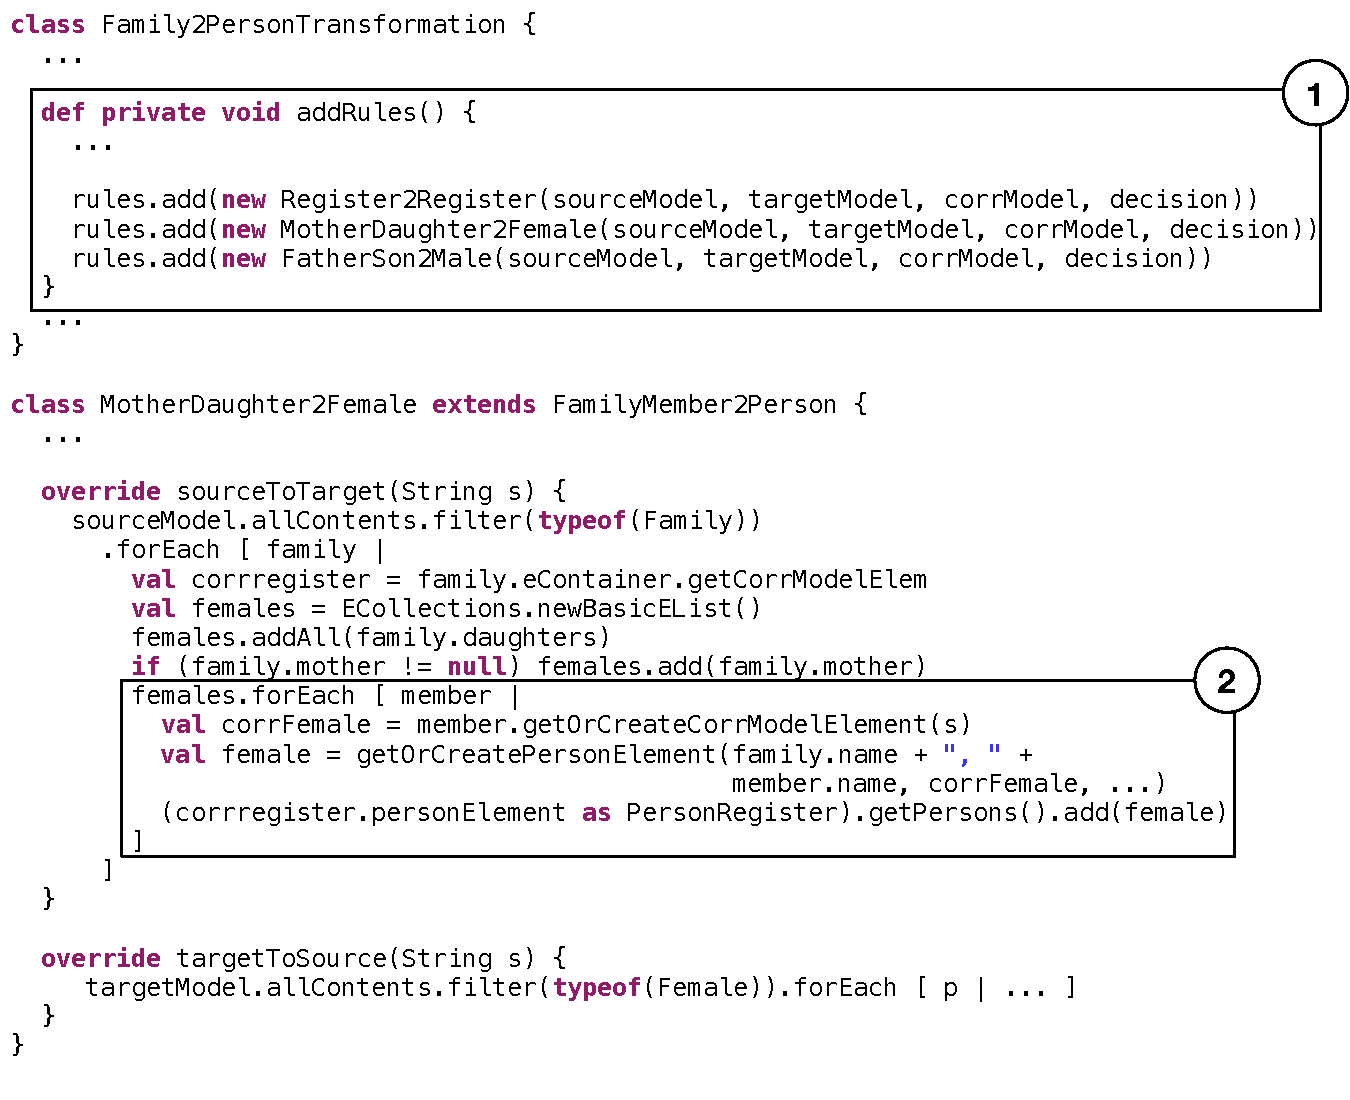
\includegraphics[width=\columnwidth]{diagrams/solutions/bxtendSoln}
    \caption{Rule orchestration and a specific rule with BXtend}
    \label{fig:bxtendSoln}
\end{figure}

The specific rule \texttt{Mother\-Daughter\-2\-Female} depicted in figure~\ref{fig:bxtendSoln} checks for and handles, as its name suggests, inconsistencies between mothers/daughters in the source model and females in the target model.
The two methods in this class \texttt{source\-To\-Target} and \texttt{target\-To\-Source} indicate that both synchronization directions (here \emph{fCR} and \emph{bCR}) are explicitly specified.
The first step in \texttt{source\-To\-Target} is to filter for all families, and to accumulate all ``female'' family members, i.e., a mother if present, and all daughters.
In the code fragment marked with label 2, the provided diag is accessed and used to retrieve the person connected to each female family member.
With a helper method \texttt{get\-Or\-Create\-Person\-Element}, this person is either created if necessary, or updated as required.
